Para facilitar el entendimiento del sistema al completo se han desarrollado dos
tipos de diagramas: los diagramas de casos de uso con sus correspondientes
explicaciones (punto \ref{ssec:use-case}) y los diagramas de bloques que modelan
al sistema en su conjunto, sus relaciones y operaciones (punto \ref{ssec:block-diagrams}).

Es importante destacar que los diagramas se quedan en una capa de abstracción por encima
de la definición de comportamiento del mismo, es decir, no se entra en excesivo detalle
sobre cómo va a hacer algo, solo especifica el qué.

\subsection{Casos de uso}\label{ssec:use-case}

A continuación se presentan los distintos diagramas de casos de uso que modelan el
comportamiento del sistema ante ciertos eventos. Se incluye además, por cada caso
de uso, una tabla adjunta que describe el caso de uso, los pasos esperados en la
secuencia normal de ejecución, las excepciones previstas durante la ejecución normal
y la resolución de las mismas.

\subsubsection{Caso de uso \texttt{01} -- autenticación}

\begin{figure}[H]
  \centering
  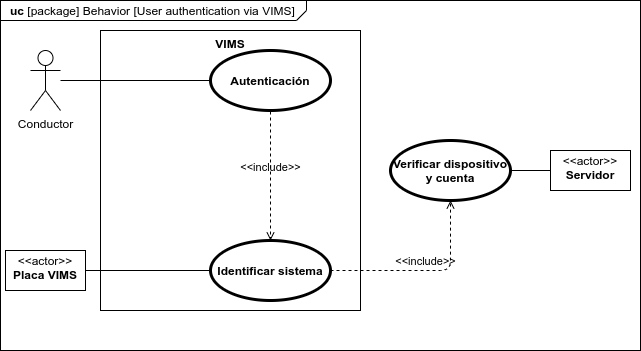
\includegraphics[width=\linewidth]{diagrams/UseCases-UC1 - auth.png}
  \caption{Caso de uso \texttt{01} -- \textit{autenticación}.}
  \label{uc:auth}
\end{figure}

\begin{table}[H]
  \centering
  \begin{tabularx}{\textwidth}{|c|c|X|}
    \hline
    \texttt{01}                                & \multicolumn{2}{c|}{\textit{Autenticación}}                                                                                                                                                                                                                 \\
    \hline
    \textbf{Descripción}                       & \multicolumn{2}{X|}{La placa identificará de forma inequívoca al conductor (usuario) y a sí misma frente al servidor.}                                                                                                                                      \\
    \hline
    \multirow{9}{*}{\textbf{Secuencia normal}} & \textbf{Paso}                                                                                                          & \textbf{Acción}                                                                                                                    \\
    \cline{2-3}
                                               & 1                                                                                                                      & \multicolumn{1}{L|}{El usuario se autentica contra la placa con su cuenta personal ya creada.}                                     \\
    \cline{2-3}
                                               & 2                                                                                                                      & \multicolumn{1}{L|}{La placa \ac{VIMS} recoge la información del usuario y la envía al servidor junto con su identificador único.} \\
    \cline{2-3}
                                               & 3                                                                                                                      & \multicolumn{1}{L|}{El servidor verifica que la cuenta del usuario existe y se asocia la información al dispositivo.}              \\
    \cline{2-3}
                                               & 4                                                                                                                      & \multicolumn{1}{L|}{La placa almacena la información del usuario y finaliza el proceso de inicio de sesión.}                       \\
    \hline
    \multirow{4}{*}{\textbf{Excepciones}}      & \textbf{Paso}                                                                                                          & \textbf{Acción}                                                                                                                    \\
    \cline{2-3}
                                               & 2                                                                                                                      & \multicolumn{1}{L|}{La placa no cuenta con conexión a la red o el servidor no está disponible.}                                    \\
    \cline{2-3}
                                               & 3                                                                                                                      & \multicolumn{1}{L|}{La cuenta del usuario no existe.}                                                                              \\
    \hline\hline
    \textbf{Resolución}                        & \multicolumn{2}{X|}{La placa funciona en modo desconectado, es decir, no transmite datos al servidor.}                                                                                                                                                      \\
    \hline
  \end{tabularx}
\end{table}

\subsubsection{Caso de uso \texttt{02} -- generación y transmisión de datos}

\begin{figure}[H]
  \centering
  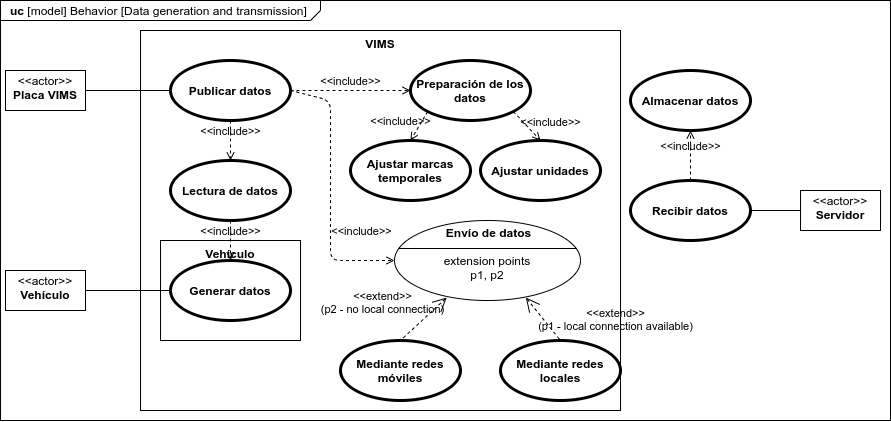
\includegraphics[width=\linewidth]{diagrams/UseCases-UC2 - data.png}
  \caption{Casos de uso \texttt{02} -- \textit{generación y transmisión de datos}.}
  \label{uc:data}
\end{figure}

\begin{table}[H]
  \centering
  \begin{tabularx}{\textwidth}{|c|c|X|}
    \hline
    \texttt{02}                                 & \multicolumn{2}{c|}{\textit{Generación y transmisión de datos}}                                                                                                                                                                                                                                                                                                                             \\
    \hline
    \textbf{Descripción}                        & \multicolumn{2}{X|}{El dispositivo \ac{VIMS} recibirá los datos del vehículo al que está conectado y los preparará para una posterior transmisión al servidor remoto de almacenamiento y gestión.}                                                                                                                                                                                          \\
    \hline
    \multirow{10}{*}{\textbf{Secuencia normal}} & \textbf{Paso}                                                                                                                                                                                                                & \textbf{Acción}                                                                                                                                              \\
    \cline{2-3}
                                                & 1                                                                                                                                                                                                                            & \multicolumn{1}{L|}{La placa \ac{VIMS} recibe los datos que el vehículo está generando de forma continuada.}                                                 \\
    \cline{2-3}
                                                & 2                                                                                                                                                                                                                            & \multicolumn{1}{L|}{Los datos recibidos se preparan para el envío, ajustando cierta información y añadiendo valores como la cuenta asociada a dichos datos.} \\
    \cline{2-3}
                                                & 3                                                                                                                                                                                                                            & \multicolumn{1}{L|}{Mediante el uso de redes móviles o locales, según disponibilidad, se envían los datos al servidor.}                                      \\
    \cline{2-3}
                                                & 4                                                                                                                                                                                                                            & \multicolumn{1}{L|}{El servidor recibe la información transmitida por el sistema y la almacena para una posterior visualización y tratamiento.}              \\
    \hline
    \multirow{9}{*}{\textbf{Excepciones}}       & \textbf{Paso}                                                                                                                                                                                                                & \textbf{Acción}                                                                                                                                              \\
    \cline{2-3}
                                                & 1                                                                                                                                                                                                                            & \multicolumn{1}{L|}{El vehículo no está conectado o no transmite datos.}                                                                                     \\
    \cline{2-3}
                                                & 2                                                                                                                                                                                                                            & \multicolumn{1}{L|}{Todavía no hay ninguna cuenta asociada a la placa \ac{VIMS}.}                                                                            \\
    \cline{2-3}
                                                & 3.1                                                                                                                                                                                                                          & \multicolumn{1}{L|}{No hay redes móviles disponibles, se intenta transmitir por redes locales.}                                                              \\
    \cline{2-3}
                                                & 3.2                                                                                                                                                                                                                          & \multicolumn{1}{L|}{No hay redes locales disponibles, se intenta transmitir por redes móviles.}                                                              \\
    \cline{2-3}
                                                & 3.3                                                                                                                                                                                                                          & \multicolumn{1}{L|}{No hay redes disponibles, se almacenan los datos para su posterior transmisión.}                                                         \\
    \hline\hline
    \textbf{Resolución}                         & \multicolumn{2}{X|}{La placa funciona en modo desconectado, es decir, no transmite datos al servidor. Si existe una cuenta asociada pero no hay conexión, los datos se almacenan en memoria hasta que se puedan transmitir.}                                                                                                                                                                \\
    \hline
  \end{tabularx}
\end{table}

\subsubsection{Caso de uso \texttt{03} -- generación de estadísticas}

\begin{figure}[H]
  \centering
  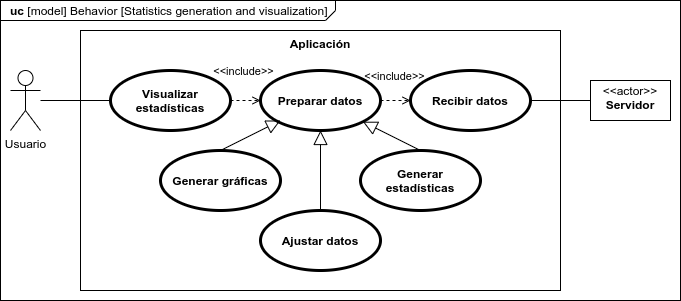
\includegraphics[width=\linewidth]{diagrams/UseCases-UC3 - stats.png}
  \caption{Caso de uso \texttt{03} -- \textit{generación de estadísticas}.}
  \label{uc:stats}
\end{figure}

\begin{table}[H]
  \centering
  \begin{tabularx}{\textwidth}{|c|c|X|}
    \hline
    \texttt{03}                                & \multicolumn{2}{c|}{\textit{Generación de estadísticas}}                                                                                                                                                                                                                                                                \\
    \hline
    \textbf{Descripción}                       & \multicolumn{2}{X|}{El servidor, en conjunción con el resto de elementos del sistema, preparará los datos para generar información estadística útil para el usuario.}                                                                                                                                                   \\
    \hline
    \multirow{7}{*}{\textbf{Secuencia normal}} & \textbf{Paso}                                                                                                                                                         & \textbf{Acción}                                                                                                                                 \\
    \cline{2-3}
                                               & 1                                                                                                                                                                     & \multicolumn{1}{L|}{El usuario solicita al servidor visualizar estadísticas con respecto a sus vehículos.}                                      \\
    \cline{2-3}
                                               & 2                                                                                                                                                                     & \multicolumn{1}{L|}{El servidor prepara los datos y genera distintos tipos de información estadística visual basados en tablas, gráficos, etc.} \\
    \cline{2-3}
                                               & 3                                                                                                                                                                     & \multicolumn{1}{L|}{El usuario recibe la información estadística ajustada a su cuenta.}                                                         \\
    \hline
    \multirow{4}{*}{\textbf{Excepciones}}      & \textbf{Paso}                                                                                                                                                         & \textbf{Acción}                                                                                                                                 \\
    \cline{2-3}
                                               & 1.1                                                                                                                                                                   & \multicolumn{1}{L|}{El usuario no está autenticado.}                                                                                            \\
    \cline{2-3}
                                               & 1.2                                                                                                                                                                   & \multicolumn{1}{L|}{El usuario no cuenta con ningún dispositivo \ac{VIMS} asociado.}                                                            \\
    \cline{2-3}
                                               & 2                                                                                                                                                                     & \multicolumn{1}{L|}{Todavía no se ha registrado ningún dato.}                                                                                   \\
    \hline\hline
    \textbf{Resolución}                        & \multicolumn{2}{X|}{Se notifica al usuario de este suceso y se le sugiere crear una cuenta.}                                                                                                                                                                                                                            \\
    \hline
  \end{tabularx}
\end{table}

\subsubsection{Caso de uso \texttt{04} -- envío de notificaciones}

\begin{figure}[H]
  \centering
  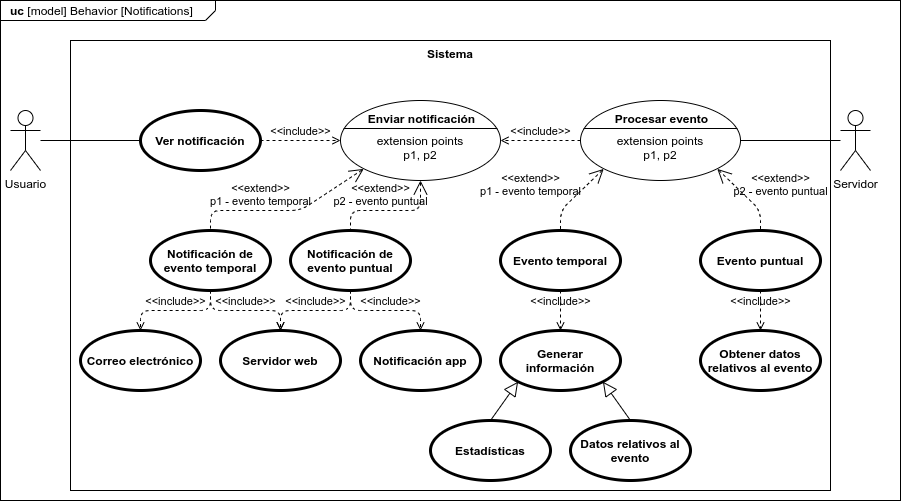
\includegraphics[width=\linewidth]{diagrams/UseCases-UC4 - notifications.png}
  \caption{Caso de uso \texttt{04} -- \textit{envío de notificaciones}.}
  \label{uc:notifications}
\end{figure}

\begin{table}[H]
  \centering
  \begin{tabularx}{\textwidth}{|c|c|X|}
    \hline
    \texttt{04}                                 & \multicolumn{2}{c|}{\textit{Envío de notificaciones}}                                                                                                                                                                                                                                                                                                                                                                                   \\
    \hline
    \textbf{Descripción}                        & \multicolumn{2}{X|}{El servidor, en conjunción con el resto de elementos del sistema, detecta ciertos eventos y actúa generando una notificación que envía al usuario.}                                                                                                                                                                                                                                                                 \\
    \hline
    \multirow{18}{*}{\textbf{Secuencia normal}} & \textbf{Paso}                                                                                                                                                           & \textbf{Acción}                                                                                                                                                                                                                                               \\
    \cline{2-3}
                                                & 1                                                                                                                                                                       & \multicolumn{1}{L|}{El servidor en un instante puntual produce y procesa un evento.}                                                                                                                                                                          \\
    \cline{2-3}
                                                & 1.1                                                                                                                                                                     & \multicolumn{1}{L|}{Si el evento se ha producido por un hecho (p.e.: repostar, finalizar un viaje, \dots), es un evento puntual sobre el cual se envía información relativa al mismo y al contexto (estadísticas del depósito, información del viaje, etc.).} \\
    \cline{2-3}
                                                & 1.2                                                                                                                                                                     & \multicolumn{1}{L|}{Si el evento se ha producido porque ha pasado un lapso de tiempo, es un evento temporal. El servidor generará estadísticas relativas a ese lapso de tiempo y mandará esa notificación.}                                                   \\
    \cline{2-3}
                                                & 2                                                                                                                                                                       & \multicolumn{1}{L|}{Se envía una notificación al usuario con los datos relativos al evento.}                                                                                                                                                                  \\
    \cline{2-3}
                                                & 2.1                                                                                                                                                                     & \multicolumn{1}{L|}{Si es un evento puntual, la notificación se envía a todos los medios: correo electrónico, servidor web y aplicación.}                                                                                                                     \\
    \cline{2-3}
                                                & 2.2                                                                                                                                                                     & \multicolumn{1}{L|}{Si es un evento temporal, la notificación se envía solo al correo electrónico y al servidor web.}                                                                                                                                         \\
    \cline{2-3}
                                                & 3                                                                                                                                                                       & \multicolumn{1}{L|}{El usuario recibe la notificación en alguno de los tres medios.}                                                                                                                                                                          \\
    \hline
  \end{tabularx}
\end{table}

\subsubsection{Caso de uso \texttt{05} -- visualización en tiempo real}

\begin{figure}[H]
  \centering
  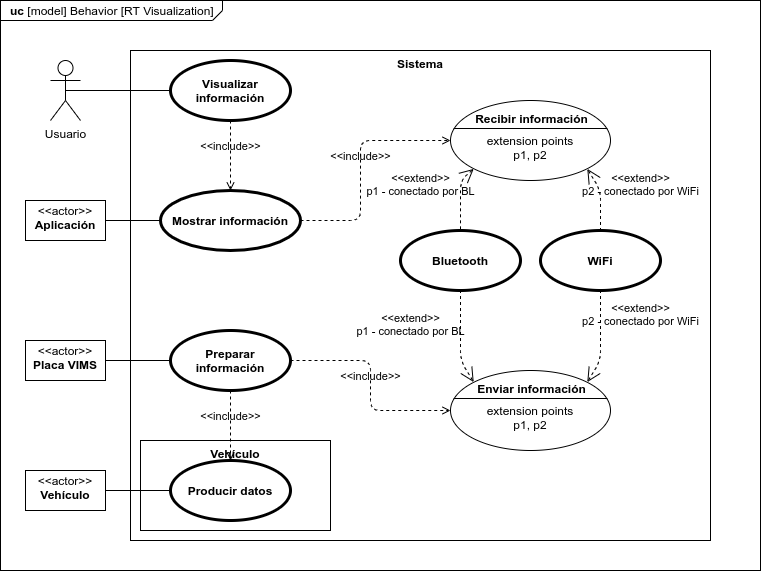
\includegraphics[width=\linewidth]{diagrams/UseCases-UC5 - visualization.png}
  \caption{Caso de uso \texttt{05} -- \textit{visualización en tiempo real}}
  \label{uc:visualization}
\end{figure}

\begin{table}[H]
  \centering
  \begin{tabularx}{\textwidth}{|c|c|X|}
    \hline
    \texttt{05}                                & \multicolumn{2}{c|}{\textit{Visualización en tiempo real}}                                                                                                                                                                                          \\
    \hline
    \textbf{Descripción}                       & \multicolumn{2}{X|}{Un usuario podrá visualizar información en tiempo real sobre su vehículo mediante la aplicación.}                                                                                                                               \\
    \hline
    \multirow{7}{*}{\textbf{Secuencia normal}} & \textbf{Paso}                                                                                                          & \textbf{Acción}                                                                                                            \\
    \cline{2-3}
                                               & 1                                                                                                                      & \multicolumn{1}{L|}{El usuario solicita visualizar información sobre el vehículo desde la aplicación.}                     \\
    \cline{2-3}
                                               & 2                                                                                                                      & \multicolumn{1}{L|}{La aplicación recibe la información de la placa \ac{VIMS} usando redes \ac{PAN}.}                      \\
    \cline{2-3}
                                               & 3                                                                                                                      & \multicolumn{1}{L|}{La placa \ac{VIMS} prepara la información que recibe del vehículo y la transmite hacia la aplicación.} \\
    \hline
    \multirow{10}{*}{\textbf{Excepciones}}     & \textbf{Paso}                                                                                                          & \textbf{Acción}                                                                                                            \\
    \cline{2-3}
                                               & 1.1                                                                                                                    & \multicolumn{1}{L|}{El usuario no está autenticado.}                                                                       \\
    \cline{2-3}
                                               & 1.2                                                                                                                    & \multicolumn{1}{L|}{El usuario no cuenta con ningún dispositivo \ac{VIMS} asociado.}                                       \\
    \cline{2-3}
                                               & 2.1                                                                                                                    & \multicolumn{1}{L|}{No hay conexión mediante Bluetooth, se realiza la comunicación por WiFi.}                              \\
    \cline{2-3}
                                               & 2.2                                                                                                                    & \multicolumn{1}{L|}{No hay conexión mediante WiFi, se realiza la comunicación por Bluetooth.}                              \\
    \cline{2-3}
                                               & 2.3                                                                                                                    & \multicolumn{1}{L|}{La placa \ac{VIMS} está desconectada.}                                                                 \\
    \cline{2-3}
                                               & 3                                                                                                                      & \multicolumn{1}{L|}{La placa \ac{VIMS} está desconectada o el vehículo no emite ningún dato.}                              \\
    \hline\hline
    \textbf{Resolución}                        & \multicolumn{2}{X|}{La placa no realiza ninguna transmisión de información hasta que no haya una conexión disponible.}                                                                                                                              \\
    \hline
  \end{tabularx}
\end{table}

\subsubsection{Caso de uso \texttt{06} -- generación de eventos}

\begin{figure}[H]
  \centering
  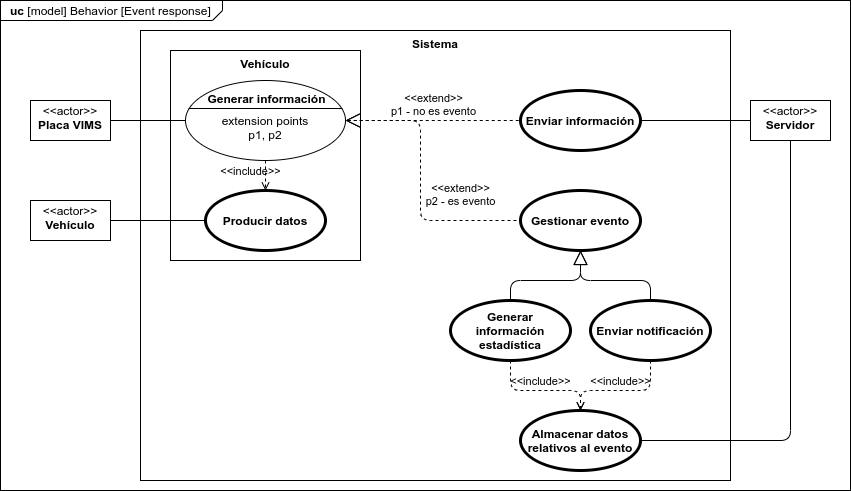
\includegraphics[width=\linewidth]{diagrams/UseCases-UC6 - reaction.png}
  \caption{Caso de uso \texttt{06} -- \textit{generación de eventos}}
  \label{uc:reaction}
\end{figure}

\begin{table}[H]
  \centering
  \begin{tabularx}{\textwidth}{|c|c|X|}
    \hline
    \texttt{06}                                 & \multicolumn{2}{c|}{\textit{Generación de eventos}}                                                                                                                                                                                                                                                                         \\
    \hline
    \textbf{Descripción}                        & \multicolumn{2}{X|}{El dispositivo \ac{VIMS}, a la hora de enviar datos, podrá producir eventos según el tipo de información que haya de enviar.}                                                                                                                                                                           \\
    \hline
    \multirow{10}{*}{\textbf{Secuencia normal}} & \textbf{Paso}                                                                                                                                     & \textbf{Acción}                                                                                                                                                         \\
    \cline{2-3}
                                                & 1                                                                                                                                                 & \multicolumn{1}{L|}{El dispositivo \ac{VIMS} genera información y la transmite hacia el servidor.}                                                                      \\
    \cline{2-3}
                                                & 1.1                                                                                                                                               & \multicolumn{1}{L|}{Si la información a transmitir es ``normal'', se envía directamente al servidor.}                                                                   \\
    \cline{2-3}
                                                & 1.2                                                                                                                                               & \multicolumn{1}{L|}{Si la información a transmitir es eventual, se procesa el evento generando información estadística referente al mismo o mandando una notificación.} \\
    \cline{2-3}
                                                & 2                                                                                                                                                 & \multicolumn{1}{L|}{El servidor recibe el evento y se encarga de gestionarlo, como se vio en el \texttt{UC-04}.}                                                        \\
    \hline
    \multirow{3}{*}{\textbf{Excepciones}}       & \textbf{Paso}                                                                                                                                     & \textbf{Acción}                                                                                                                                                         \\
    \cline{2-3}
                                                & 1                                                                                                                                                 & \multicolumn{1}{L|}{No hay ninguna cuenta asociada al dispositivo.}                                                                                                     \\
    \cline{2-3}
                                                & 1.1                                                                                                                                               & \multicolumn{1}{L|}{No hay conexión a Internet por parte del dispositivo \ac{VIMS}.}                                                                                    \\
    \hline\hline
    \textbf{Resolución}                         & \multicolumn{2}{X|}{La placa funciona en modo desconectado, es decir, no transmite datos al servidor.}                                                                                                                                                                                                                      \\
    \hline
  \end{tabularx}
\end{table}

\subsubsection{Caso de uso \texttt{07.*} -- envío, almacenamiento y visualización de geolocalización}

\begin{figure}[H]
  \centering
  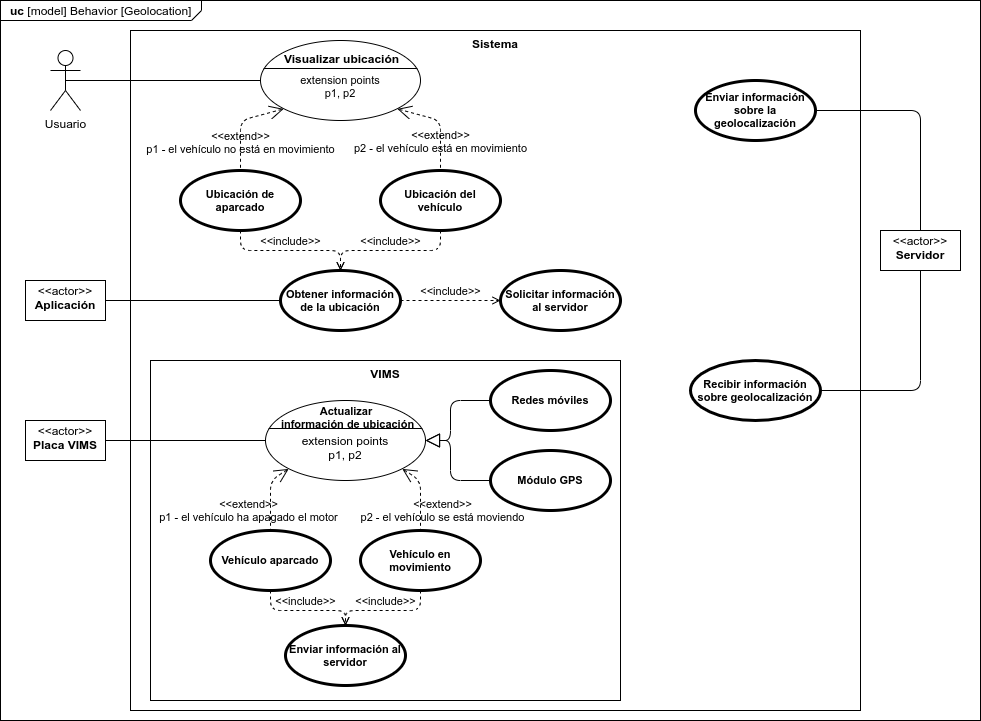
\includegraphics[width=\linewidth]{diagrams/UseCases-UC7 - location.png}
  \caption{Casos de uso \texttt{07.*} -- \textit{envío, almacenamiento y visualización de geolocalización}}
  \label{uc:location}
\end{figure}

\begin{table}[H]
  \centering
  \begin{tabularx}{\textwidth}{|c|c|X|}
    \hline
    \texttt{07.1}                               & \multicolumn{2}{c|}{\textit{Visualización de ubicación}}                                                                                                                                                                                                                                                                                                        \\
    \hline
    \textbf{Descripción}                        & \multicolumn{2}{X|}{El usuario mediante una aplicación podrá visualizar la ubicación del vehículo en tiempo real. Si el vehículo está apagado, se visualiza la ubicación del aparcamiento.}                                                                                                                                                                     \\
    \hline
    \multirow{10}{*}{\textbf{Secuencia normal}} & \textbf{Paso}                                                                                                                                                                               & \textbf{Acción}                                                                                                                                                   \\
    \cline{2-3}
                                                & 1                                                                                                                                                                                           & \multicolumn{1}{L|}{El usuario inicia una aplicación para visualizar la ubicación de su vehículo.}                                                                \\
    \cline{2-3}
                                                & 1.1                                                                                                                                                                                         & \multicolumn{1}{L|}{Si el vehículo se encuentra en movimiento, se visualiza la ubicación en tiempo real según se va actualizando.}                                \\
    \cline{2-3}
                                                & 1.2                                                                                                                                                                                         & \multicolumn{1}{L|}{Si el vehículo está apagado se considera que está aparcado y se visualiza la última ubicación conocida, correspondiente con el aparcamiento.} \\
    \cline{2-3}
                                                & 2                                                                                                                                                                                           & \multicolumn{1}{L|}{Se realizan peticiones al servidor para obtener la información de la geolocalización.}                                                        \\
    \hline
    \multirow{3}{*}{\textbf{Excepciones}}       & \textbf{Paso}                                                                                                                                                                               & \textbf{Acción}                                                                                                                                                   \\
    \cline{2-3}
                                                & 1                                                                                                                                                                                           & \multicolumn{1}{L|}{No hay ningún dispositivo asociado a la cuenta.}                                                                                              \\
    \cline{2-3}
                                                & 1.1                                                                                                                                                                                         & \multicolumn{1}{L|}{El vehículo está desconectado de la red, por lo que no se pueden transmitir los datos de geolocalización.}                                    \\
    \cline{2-3}
                                                & 1.2                                                                                                                                                                                         & \multicolumn{1}{L|}{No hay ningún dato de geolocalización almacenado.}                                                                                            \\
    \cline{2-3}
                                                & 2                                                                                                                                                                                           & \multicolumn{1}{L|}{La aplicación no cuenta con conexión a la red.}                                                                                               \\
    \hline\hline
    \textbf{Resolución}                         & \multicolumn{2}{X|}{La placa funciona en modo desconectado, es decir, no transmite datos al servidor.}                                                                                                                                                                                                                                                          \\
    \hline
  \end{tabularx}
\end{table}

\begin{table}[H]
  \centering
  \begin{tabularx}{\textwidth}{|c|c|X|}
    \hline
    \texttt{07.2}                               & \multicolumn{2}{c|}{\textit{Envío de ubicación}}                                                                                                                                                                                                                                                 \\
    \hline
    \textbf{Descripción}                        & \multicolumn{2}{X|}{La placa \ac{VIMS} enviará la información relativa al vehículo al servidor.}                                                                                                                                                                                                 \\
    \hline
    \multirow{18}{*}{\textbf{Secuencia normal}} & \textbf{Paso}                                                                                    & \textbf{Acción}                                                                                                                                                                               \\
    \cline{2-3}
                                                & 1                                                                                                & \multicolumn{1}{L|}{La placa actualiza la información sobre la ubicación del vehículo.}                                                                                                       \\
    \cline{2-3}
                                                & 1.1                                                                                              & \multicolumn{1}{L|}{Si se ha perdido la conexión con el vehículo (motor apagado), se considera que está aparcado y se envía la ubicación actual como ``ubicación de aparcado''.}              \\
    \cline{2-3}
                                                & 1.2                                                                                              & \multicolumn{1}{L|}{Si el vehículo está activo (motor encendido), se considera que está en movimiento y envía de forma periódica la ubicación actual del vehículo.}                           \\
    \cline{2-3}
                                                & 2                                                                                                & \multicolumn{1}{L|}{Según la precisión de las redes y la disponibilidad de las mismas, la ubicación se obtiene mediante dos métodos.}                                                         \\
    \cline{2-3}
                                                & 2.1                                                                                              & \multicolumn{1}{L|}{Se obtiene la ubicación mediante el uso de redes móviles cuando el módulo GPS no se encuentre disponible o no se tengan suficientes satélites.}                           \\
    \cline{2-3}
                                                & 2.2                                                                                              & \multicolumn{1}{L|}{Se obtiene la ubicación mediante el módulo GPS como primera alternativa, y se usan las redes móviles cuando estén disponibles para mejorar la precisión de la ubicación.} \\
    \cline{2-3}
                                                & 3                                                                                                & \multicolumn{1}{L|}{Se manda la ubicación obtenida al servidor y se enlaza a la cuenta asociada.}                                                                                             \\
    \hline
    \multirow{6}{*}{\textbf{Excepciones}}       & \textbf{Paso}                                                                                    & \textbf{Acción}                                                                                                                                                                               \\
    \cline{2-3}
                                                & 1                                                                                                & \multicolumn{1}{L|}{No hay ninguna cuenta asociada al dispositivo.}                                                                                                                           \\
    \cline{2-3}
                                                & 1.1                                                                                              & \multicolumn{1}{L|}{No hay ninguna conectividad de red disponible para realizar el envío de la ubicación.}                                                                                    \\
    \cline{2-3}
                                                & 3                                                                                                & \multicolumn{1}{L|}{La conexión de red no está disponible para realizar la transmisión de la información.}                                                                                    \\
    \hline\hline
    \textbf{Resolución}                        & \multicolumn{2}{X|}{La placa funciona en modo desconectado, es decir, no transmite datos al servidor.}                                                                                                                                                      \\
    \hline
  \end{tabularx}
\end{table}

\begin{table}[H]
  \centering
  \begin{tabularx}{\textwidth}{|c|c|X|}
    \hline
    \texttt{07.3}                              & \multicolumn{2}{c|}{\textit{Almacenamiento de los datos de ubicación}}                                                                                                                                                                                                        \\
    \hline
    \textbf{Descripción}                       & \multicolumn{2}{X|}{El servidor almacenará y gestionará los datos de ubicación recibidos por los múltiples dispositivos \ac{VIMS}.}                                                                                                                                           \\
    \hline
    \multirow{8}{*}{\textbf{Secuencia normal}} & \textbf{Paso}                                                                                                                       & \textbf{Acción}                                                                                                                         \\
    \cline{2-3}
                                               & 1                                                                                                                                   & \multicolumn{1}{L|}{El servidor recibe la información de la ubicación de un dispositivo \ac{VIMS}.}                                     \\
    \cline{2-3}
                                               & 1.1                                                                                                                                 & \multicolumn{1}{L|}{Los datos de ubicación se almacenan en una línea temporal para poder ver el histórico de ubicaciones del vehículo.} \\
    \cline{2-3}
                                               & 1.2                                                                                                                                 & \multicolumn{1}{L|}{El último valor de ubicación se almacena para una posterior visualización.}                                         \\
    \cline{2-3}
                                               & 2                                                                                                                                   & \multicolumn{1}{L|}{El servidor ofrece los datos de ubicación a través de la \ac{API}.}                                                 \\
    \hline
    \multirow{2}{*}{\textbf{Excepciones}}      & \textbf{Paso}                                                                                                                       & \textbf{Acción}                                                                                                                         \\
    \cline{2-3}
                                               & 1                                                                                                                                   & \multicolumn{1}{L|}{No hay ninguna cuenta asociada al dispositivo.}                                                                     \\
    \hline\hline
    \textbf{Resolución}                        & \multicolumn{2}{X|}{La placa funciona en modo desconectado, es decir, no transmite datos al servidor.}                                                                                                                                                      \\
    \hline
  \end{tabularx}
\end{table}

\subsection{Diagramas de bloques}\label{ssec:block-diagrams}

Los diagramas de bloques ofrecen una visión genérica del sistema en su conjunto. Para
este sistema, se han definido tres diagramas de bloques: el primero define \textit{grosso modo}
cómo se compone el sistema embebido que irá en el vehículo, con sus respectivos
componentes y condiciones; el segundo, define la arquitectura del servidor, las conexiones
con la base de datos y la \ac{API} para consulta de datos externa. Finalmente, el
tercer diagrama muestra cómo es todo el sistema en su conjunto, uniendo \ac{VIMS}
con el servidor.

\begin{figure}[H]
  \centering
  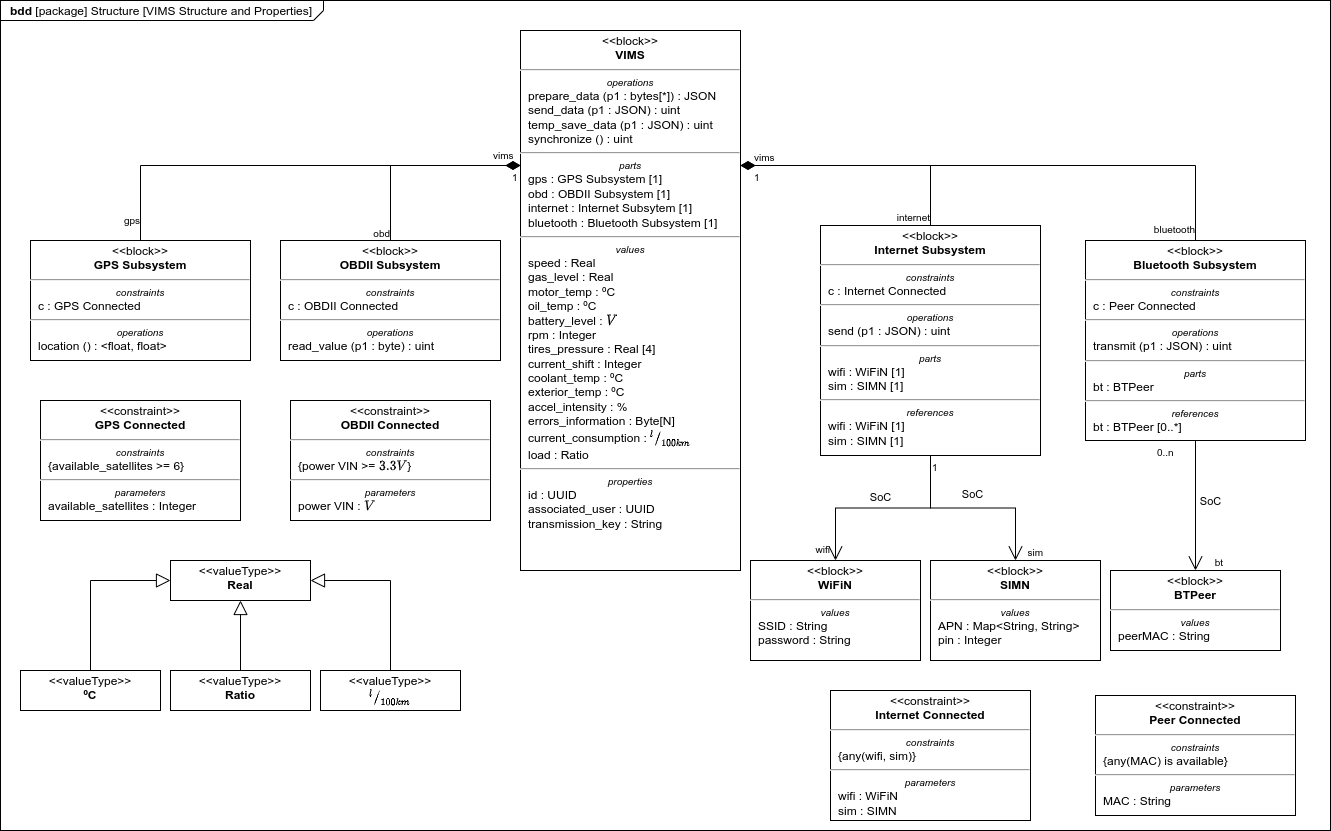
\includegraphics[width=\linewidth]{images/BlockDiagrams-VIMS.drawio.png}
  \caption{Diagrama de bloques que modela el conjunto de la placa \ac{VIMS} y sus componentes.}
  \label{bd:vims}
\end{figure}

Por una parte, se puede observar en la figura \ref{bd:vims} cómo está compuesta la placa.
Se distinguen los siguientes componentes principales:

\begin{itemize}
  \item El dispositivo \ac{VIMS} en sí, con sus funciones básicas y los datos que
        almacenará.
  \item El subsistema de conexionado \ac{GPS}, encargado de devolver la ubicación
        del sistema al que se conecta.
  \item El subsistema de conexionado \ac{OBD}--II, encargado de obtener en bytes
        los datos generados por el vehículo.
  \item El subsistema de conexionado a Internet, encargado de escoger adecuadamente
        el módulo de conexión a la red adecuado según las circunstancias del sistema
        y de realizar las comunicaciones de red.
  \item El subsistema de conexionado Bluetooth, cuya funcionalidad es la de conectarse
        a un dispositivo externo y realizar una emisión en el momento de los datos
        enviados por el vehículo.
\end{itemize}

Se va a empezar comentando cada uno de los subsistemas. Por su parte, el subsistema
\ac{GPS} (figura \ref{fig:bd-gps}) cuenta con una restricción ``\textit{GPS Connected}''
que define cuándo se considera que hay conexión con \ac{GPS}. Este valor se establece
en 6 satélites para resolver el problema del eje $Z$ que existe en trilateración con
3 satélites. En principio, con 4 satélites se podría considerar que hay conexión
con el \ac{GPS} pero con una redundancia del doble se obtiene una precisión de
aproximadamente $5~m$.

Este subsistema devuelve la latitud y la longitud, expresadas como números en coma
flotante de 32 bits (que dota al sistema de una precisión máxima de siete dígitos
decimales).

\begin{figure}[H]
  \centering
  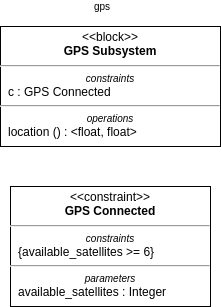
\includegraphics[width=.3\linewidth]{images/BD-GPS.png}
  \caption{Subsistema que define las comunicaciones usando el \ac{GPS} para obtener la ubicación.}
  \label{fig:bd-gps}
\end{figure}

El subsistema de \ac{OBD}--II (figura \ref{fig:bd-obd}) se encarga de la conexión con
el vehículo y remite los datos al sistema principal. La función \texttt{read\_value}
recibe un byte que se correspondería al \ac{PID} y devuelve los bytes con los datos
asociados. Al igual que el subsistema anterior, se plantea la restricción de que
el \ac{OBD}--II esté desconectado. Esto se hará confirmando que el $V_{in} \ge 3.3V$
aunque, en la vida real, esta restricción no existe dado que el sistema \ac{OBD}--II
del vehículo siempre ofrece un voltaje de alimentación de $12V$ en el conector (sin embargo, se ha contemplado
porque existe la posibilidad de que la placa esté encendida mediante USB sin
conexión al vehículo).

\begin{figure}[H]
  \centering
  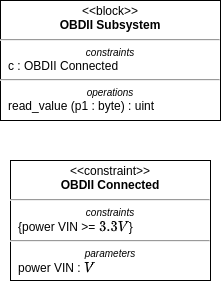
\includegraphics[width=.3\linewidth]{images/BD-OBD.png}
  \caption{Subsistema que define las comunicaciones con el vehículo usando \ac{OBD}--II.}
  \label{fig:bd-obd}
\end{figure}

El siguiente subsistema se encarga de la conectividad de red (figura \ref{fig:bd-internet}).
Contiene dos elementos ``\texttt{WiFiN}'' y ``\texttt{SIMN}'' en donde el primero
provee de conectividad WiFi y el segundo de conectividad \ac{LTE}. Este subsistema
cuenta con un único método que le permite enviar datos en forma JSON al exterior,
ya que es lo más compatible. Sin embargo, lo más importante es que se encarga de
escoger según disponibilidad un sistema u otro. Esto se realiza comprobando que
tienen acceso a la red según orden de prioridad: primero WiFi y luego SIM.

Individualmente, cada componente tiene las propiedades necesarias para conectarse.
Por su parte, la conexión WiFi contiene información sobre el SSID y la contraseña.
Mientras, la conexión \ac{LTE} (SIM) almacena los datos del APN y del pin de
desbloqueo de la SIM.

La restricción para que este subsistema se considere activo es que disponga de al
menos una conexión activa y funcional.

\begin{figure}[H]
  \centering
  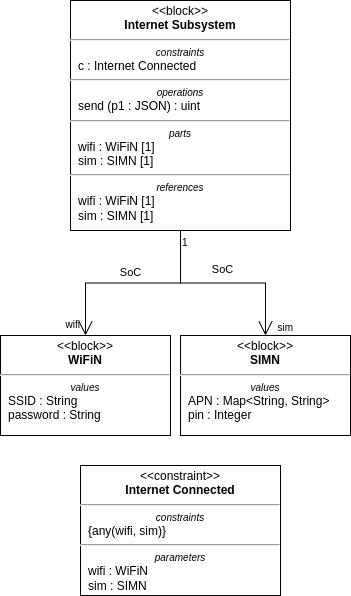
\includegraphics[width=.5\linewidth]{images/BD-Internet.png}
  \caption{Subsistema que define las comunicaciones de red con el exterior.}
  \label{fig:bd-internet}
\end{figure}

El último subsistema que forma parte de \ac{VIMS} es aquél que provee de conectividad
Bluetooth (figura \ref{fig:bd-bluetooth}). Este subsistema funciona en principio
usando \ac{BLE} por lo que es posible conectar múltiples dispositivos a la vez. Sin
embargo, por restricciones del proyecto se limita a una única conexión simultánea.
Por cada elemento emparejado, se almacena su dirección MAC para realizar la conexión
de nuevo.

Además, este subsistema tiene una restricción que define si está conectado si alguna
MAC almacenada está disponible y aceptando conexiones.

\begin{figure}[H]
  \centering
  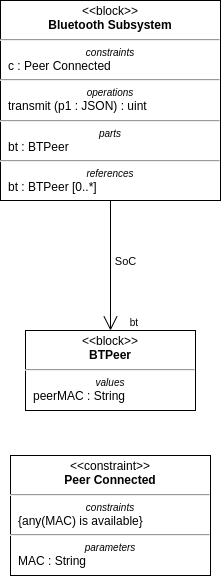
\includegraphics[width=.3\linewidth]{images/BD-Bluetooth.png}
  \caption{Subsistema de conexionado Bluetooth para la transmisión en vivo de los datos.}
  \label{fig:bd-bluetooth}
\end{figure}

Finalmente, queda el sistema principal: \ac{VIMS} que congrega al resto de subsistemas
y hace uso de las funcionalidades que ofrecen (figura \ref{fig:bd-vims}).

\begin{figure}[H]
  \centering
  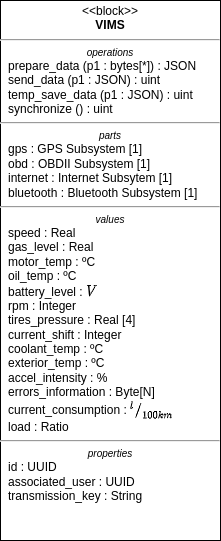
\includegraphics[width=.3\linewidth]{images/BD-VIMS.png}
  \caption{Componente \ac{VIMS} dentro del sistema embebido.}
  \label{fig:bd-vims}
\end{figure}

Este sistema se congrega de los subsistemas definidos anteriormente y define múltiples
métodos que realizan una serie de operaciones con los mismos. Por una parte, \texttt{prepare\_data}
prepara los valores recibidos en crudo por el subsistema \ac{OBD} para su posterior
transmisión. Esta operación realiza las conversiones adecuadas de los valores en
bytes, ajusta las unidades de los mismos y lo guarda en los campos correspondientes
definidos en ``\textit{values}''.

Por otra parte, la función \texttt{send\_data} envía los valores previamente preparados
al servidor remoto de gestión. El valor de retorno de esta operación es un código
entero que identifica la respuesta del servidor ante la transmisión.

Si por un casual el subsistema de conexión a Internet no se encuentra disponible
(es decir, no hay ni conexión WiFi ni SIM), existe la función \texttt{temp\_save\_data}
que almacenará los datos temporalmente en memoria persistente, hasta que se cuente
con conexión a la red.

Finalmente, existe la función \texttt{synchronize} que se encargará de mantener
actualizados los datos que se muestran en el dispositivo del usuario cuando dicho
dispositivo está conectado por Bluetooth y está en modo de monitorización.

En lo referente a los valores del bloque, se corresponden a los distintos datos que
serán accedidos usando el subsistema \ac{OBD} y que se guardan como referencia para
su posterior transmisión. No se va a entrar en detalle en explicar qué dato es cada
uno de los mostrados. Referirse a la sección \ref{sec:hardware} para más detalles.

Por último, en el apartado de propiedades, se almacenan todos aquellos valores
que identifican el dispositivo \ac{VIMS} en sí y la cuenta de usuario asociada
al mismo (junto con su clave de transmisión). Cada dispositivo \ac{VIMS} deberá
poder ser identificado de manera inequívoca y existe la posibilidad de que un mismo
usuario tenga múltiples dispositivos \ac{VIMS}. Como hay cierta información que
se puede considerar sensible, se genera una clave de transmisión asociada a la
cuenta y al dispositivo que permitirá asegurar la integridad, inmutabilidad y
confidencialidad de los datos durante la transmisión.

Estos valores se almacenan durante el primer arrancado del dispositivo. Según los
casos de uso (\ref{ssec:use-case}), el dispositivo \ac{VIMS} no hará nada mientras
esos campos no hayan sido cumplimentados, impidiendo cualquier operación con el
mismo.

\begin{figure}[H]
  \centering
  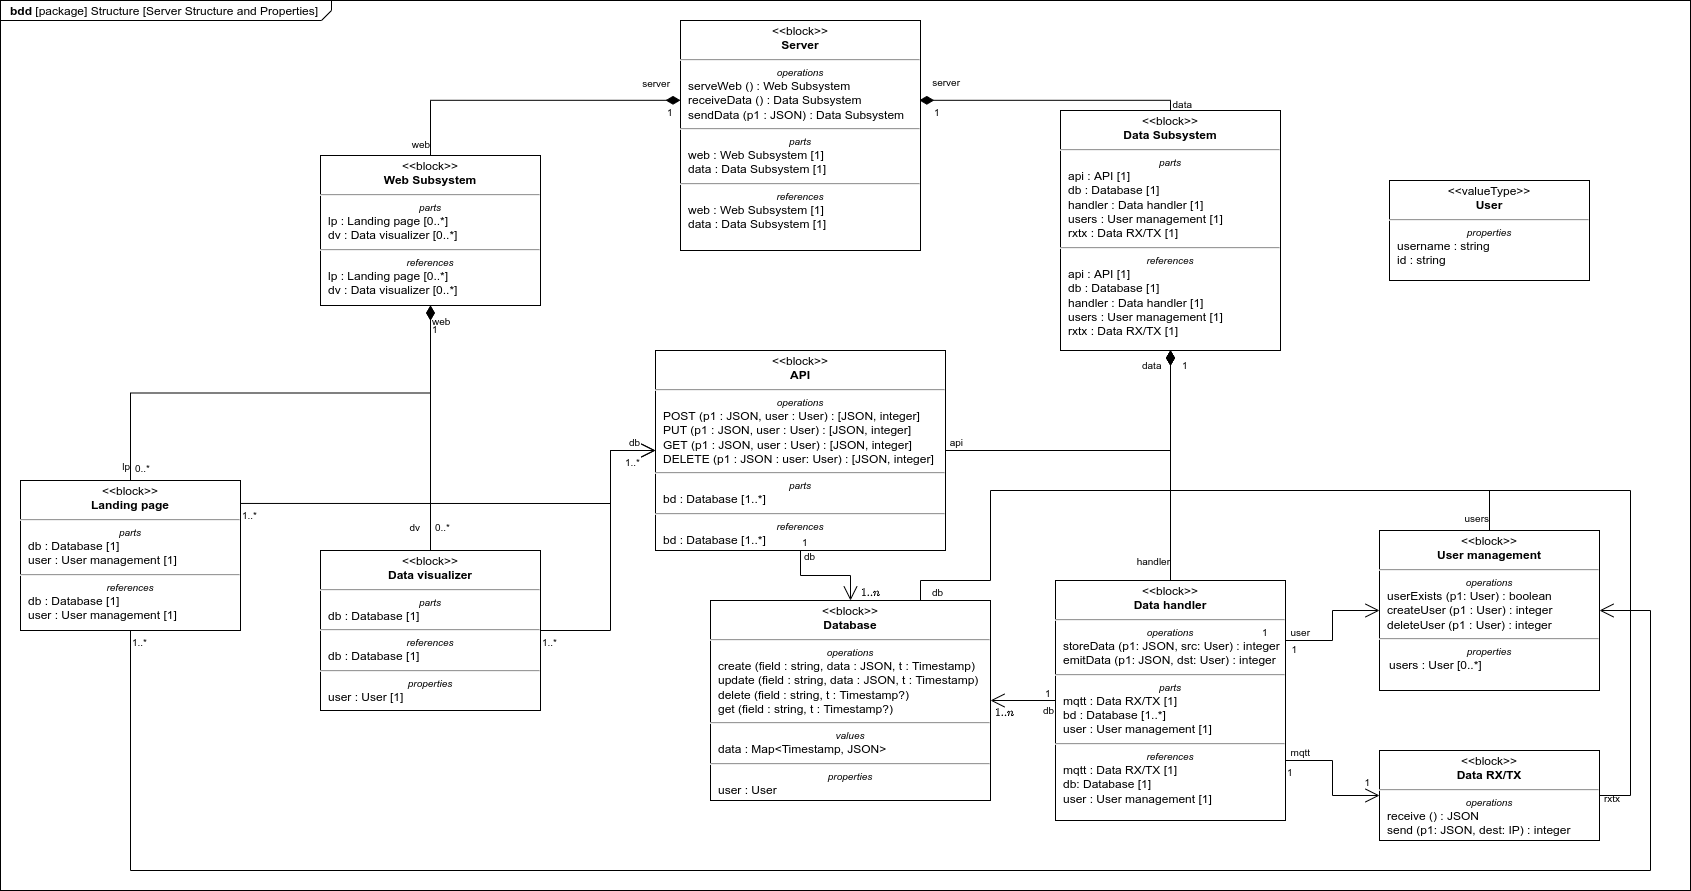
\includegraphics[width=\linewidth]{images/BlockDiagrams-Server.drawio.png}
  \caption{Diagrama de bloques que modela al servidor y sus componentes.}
  \label{bd:server}
\end{figure}

La arquitectura definida en el lado del servidor cuenta con menos componentes pero
más segregados:

\begin{itemize}
  \item El subsistema de la web, que define aquellos elementos que conforman la
        web con la que un usuario interactuará. Por una parte, existe una
        ``\textit{landing page}'' que permite que los usuarios se registren y
        creen sus cuentas. Por otro lado, se cuenta también con un visualizador
        de datos en donde el usuario podrá acceder a los últimos reportes
        sobre sus viajes y dispositivos, además de realizar las gestiones propias
        sobre su cuenta.
  \item El subsistema de datos, que engloba toda la gestión de la información
        por parte del servidor. Este subsistema se compone de una base de datos
        de almacenamiento de la información de usuario así como de los datos
        transmitidos por los dispositivos \ac{VIMS}. Otro bloque que lo conforma
        es el de gestión de la información el cual relacionará los datos recibidos
        por los dispositivos \ac{VIMS} con el usuario que los transmite. Finalmente,
        está el bloque de la \ac{API} que relaciona los dos subsistemas: accede a la
        información de manera segura almacenada en el bloque de los datos y se la
        ofrece al subsistema de la web y, en un futuro, al sistema de la aplicación
        móvil.
\end{itemize}

Toda esta arquitectura se ejecutará en un servicio en la nube que congregará y
simplificará las operaciones de mantenimiento y escalabilidad del sistema. Antes
de continuar, se va a analizar cada subsistema individualmente.

El subsistema de la web (figura \ref{fig:bd-web}) se compone de dos bloques principalmente:
un ``\textit{landing page}'' y un visualizador de datos. El primero de ellos, siguiendo
el flujo de operación definido en los casos de uso (\ref{ssec:use-case}), será
lo que un usuario arbitrario se encuentre cuando pretenda acceder al sistema por
primera vez. Allí, el usuario tendrá la capacidad de registrarse, almacenar sus
datos y registrar algún dispositivo \ac{VIMS}, si lo tiene. Como el servidor se
ejecuta en una nube alquilada, se plantea un modelo de suscripción libre en donde
un usuario puede decidir pagar una cuota mensual para acceder a las funcionalidades
del servidor.

Por otra parte, el visualizador de datos será la pantalla habitual que se encuentre un
usuario ya registrado. Allí se mostrará de forma agrupada y ordenada los datos
almacenados hasta el momento de los vehículos asociados a su cuenta (con una
estructura similar a la mostrada en la figura \ref{fig:data-ui}). Además del acceso
a los datos, el usuario podrá configurar sus preferencias, modalidad de suscripción,
dispositivos asociados, etc.

\begin{figure}[H]
  \centering
  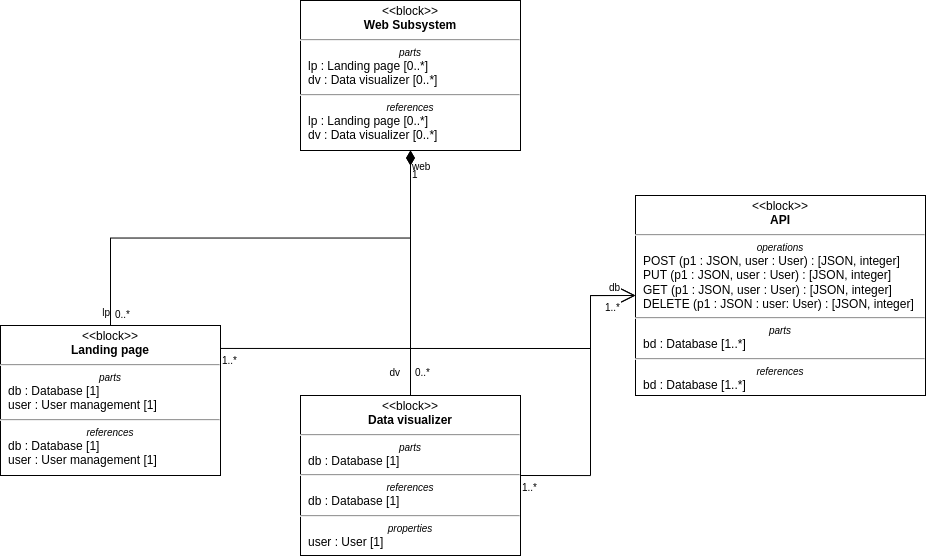
\includegraphics[width=.8\linewidth]{images/BD-web.png}
  \caption{Subsistema del servidor que conforma la arquitectura web del mismo.}
  \label{fig:bd-web}
\end{figure}

El subsistema de los datos (figura \ref{fig:bd-data}) cuenta con múltiples componentes
que lo conforman. El más básico de ellos que es usado por los demás es la base de datos.
Las operaciones definidas para dicha base de datos son \ac{CRUD}. La particularidad
de la base de datos es que cada ``instancia'' tiene asociada una cuenta de usuario,
de manera que las operaciones a realizar sobre la misma serán siempre con el usuario
como clave principal. Debido a los datos que se van a almacenar (que responden a
series temporales), el sistema propuesto de base de datos es una mezcla relacional y
no relacional. La primera se usará para almacenar toda la información que identifica
a los usuarios y sus características, que es un componente que está definido y es
limitado. Además, se almacenarán en esa base de datos toda aquella información
relacionada con las estadísticas del viaje, ya que es también una característica
inmutable. La segunda se usará para almacenar la información transmitida por los
dispositivos \ac{VIMS} dado que es una serie temporal. Se guardarán también datos
derivados de dicha transmisión y otra información de utilidad que pueda ser usada
posteriormente para generar perfiles de conducción, estadísticas, tendencias, etc.

Por otra parte, existe otro conjunto de bloques que representan las distintas
interacciones que puedan existir con los datos. Hay un bloque genérico llamado
``\textit{Data handler}'' que engloba las operaciones de escritura de los usuarios
y de los datos recibidos por los distintos dispositivos \ac{VIMS}. Este a su vez
se compone del bloque ``\textit{User management}'' que engloba las operaciones
de creación, lectura y eliminación de usuarios. El otro bloque es ``\textit{Data RX/TX}''
que se encarga de recibir los datos de los dispositivos \ac{VIMS} mediante el protocolo
MQTT. Además, también realizará las transmisiones hacia los dispositivos cuando
sea necesario (validar el usuario, actualizaciones de \textit{firmware}, \dots).

Finalmente, se encuentra el bloque de la \ac{API}. En particular, es una \ac{API} \ac{REST}
que permite realizar diversas operaciones sobre los datos asociados a una cuenta de
usuario. Al usar un sistema ampliamente estandarizado permite la interacción
directa de diversos sistemas como son \ac{VIMS}, el servidor en sí y la aplicación
móvil.

\begin{figure}[H]
  \centering
  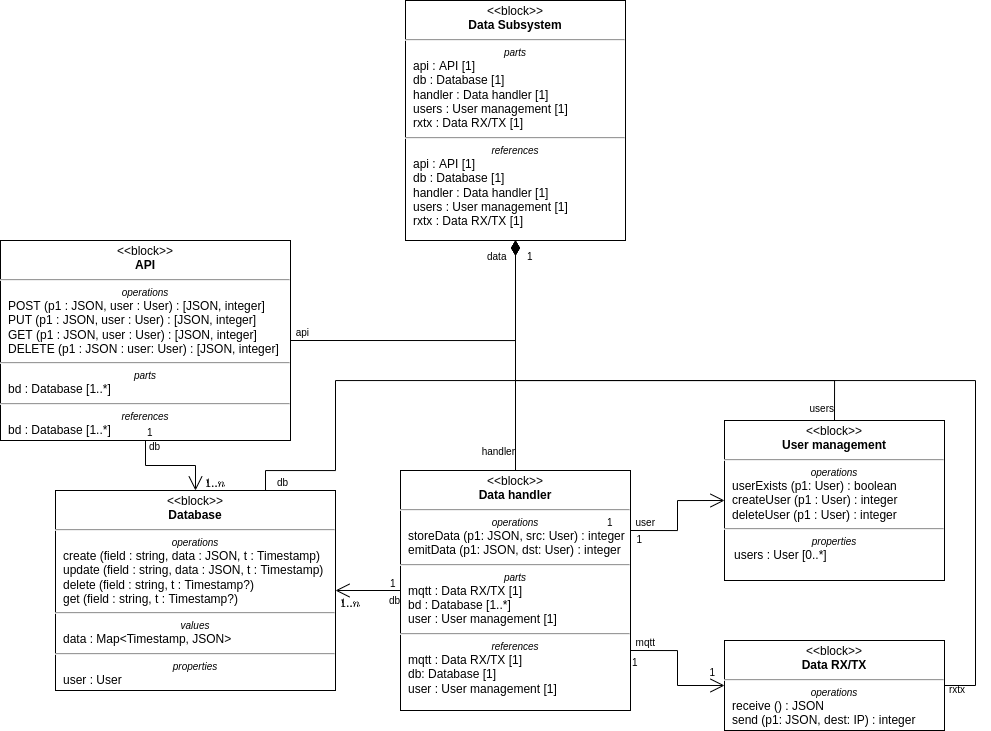
\includegraphics[width=\linewidth]{images/BD-data.png}
  \caption{Subsistema del servidor que conforma la gestión de datos y usuarios.}
  \label{fig:bd-data}
\end{figure}

Por último, se cuenta con un último diagrama que relaciona cómo funcionan los dos
esquemas de bloques anteriores (figura \ref{bd:global}):

\begin{figure}[H]
  \centering
  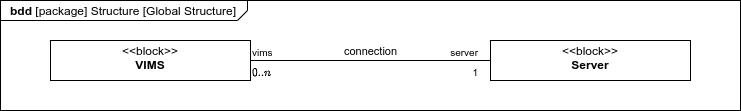
\includegraphics[width=\linewidth]{images/BlockDiagrams-Global.drawio.png}
  \caption{Diagrama global del sistema. Como se puede ver, se sigue una arquitectura cliente--servidor.}
  \label{bd:global}
\end{figure}

Como se puede observar, la multiplicidad contempla que hayan múltiples sistemas
\ac{VIMS} conectados y funcionando contra un único servidor (indiferentemente de
que, por razones de escalabilidad, este esté distribuido).
